\documentclass[UTF8]{article}
\usepackage{graphicx}
\usepackage{subfigure}
\usepackage{amsmath}
\usepackage{makecell}
\usepackage[utf8]{inputenc}
\usepackage[space]{ctex} %中文包
\usepackage{listings} %放代码
\usepackage{xcolor} %代码着色宏包
\usepackage{CJK} %显示中文宏包
\usepackage{float}
\usepackage{makecell}
\usepackage{diagbox}
\usepackage{bm}
\usepackage{ulem} 
\usepackage{amssymb}
\usepackage{soul}
\usepackage{color}
\usepackage{geometry}
\usepackage{fancybox} %花里胡哨的盒子
\usepackage{xhfill} %填充包, 可画分割线 https://www.latexstudio.net/archives/8245
\usepackage{multicol} %多栏包
\usepackage{enumerate} %可以方便地自定义枚举标题
\usepackage{multirow} %表格中多行单元格合并
\usepackage{wasysym} %可以使用wasysym里的一堆奇奇怪怪的符号
%\usepackage{mips}

\geometry{left = 2.5cm, right = 2.5cm}

\definecolor{mygreen}{rgb}{0,0.6,0}
\definecolor{mygray}{rgb}{0.5,0.5,0.5}
\definecolor{mymauve}{rgb}{0.58,0,0.82}

\lstset{
	backgroundcolor=\color{white}, 
	%\tiny < \scriptsize < \footnotesize < \small < \normalsize < \large < \Large < \LARGE < \huge < \Huge
	basicstyle = \scriptsize,       
	breakatwhitespace = false,        
	breaklines = true,                 
	captionpos = b,                    
	commentstyle = \color{mygreen}\bfseries,
	escapeinside=``,
	extendedchars = false,
	frame = shadowbox, 
	framerule=0.5pt,
	keepspaces=true,
	keywordstyle=\color{blue}\bfseries, % keyword style
	language = verilog,                     % the language of code
	otherkeywords={string}, 
	numbers=left, 
	numbersep=5pt,
	numberstyle=\tiny\color{mygray},
	rulecolor=\color{black},         
	showspaces=false,  
	showstringspaces=false, 
	showtabs=false,    
	stepnumber=1,         
	stringstyle=\color{mymauve},        % string literal style
	tabsize=4,          
	title=\lstname,
	texcl=true  
}

%\sum\nolimits_{j=1}^{M}   上下标位于求和符号的水平右端,
%\sum\limits_{j=1}^{M}   上下标位于求和符号的上下处,
%\sum_{j=1}^{M}  对上下标位置没有设定,会随公式所处环境自动调整。

%%%%%%%%%%%%%画图包%%%%%%%%%%%%%
\usepackage{tikz}
%%%%%%%%%%%%%画图背景包%%%%%%%%%%%%%
\usetikzlibrary{backgrounds}

%%%%%%%%%%%%%在tikz中画一个顶点%%%%%%%%%%%%%
%%%%%%%%%%%%%#1:node名称%%%%%%%%%%%%%
%%%%%%%%%%%%%#2:位置%%%%%%%%%%%%%
%%%%%%%%%%%%%#3:标签%%%%%%%%%%%%%
\newcommand{\newVertex}[3]{\node[circle, draw=black, line width=1pt, scale=0.8] (#1) at #2{#3}}
%%%%%%%%%%%%%在tikz中画一条边%%%%%%%%%%%%%
\newcommand{\newEdge}[2]{\draw [black,very thick](#1)--(#2)}
%%%%%%%%%%%%%在tikz中放一个标签%%%%%%%%%%%%%
%%%%%%%%%%%%%#1:名称%%%%%%%%%%%%%
%%%%%%%%%%%%%#2:位置%%%%%%%%%%%%%
%%%%%%%%%%%%%#3:标签内容%%%%%%%%%%%%%
\newcommand{\newLabel}[3]{\node[line width=1pt] (#1) at #2{#3}}

%%%%%%%%%%%%%强制跳过一行%%%%%%%%%%%%%
\newcommand{\jumpLine} {\hspace*{\fill} \par}
%%%%%%%%%%%%%关键点指令,可用itemise替代%%%%%%%%%%%%%
\newcommand{\average}[1]{\left\langle #1\right\rangle }
%%%%%%%%%%%%%表格内嵌套表格%%%%%%%%%%%%%

\newcommand{\keypoint}[2]{$\bullet$\textbf{#1}\quad#2\par}
%%%%%%%%%%%%%<T>平均值表示%%%%%%%%%%%%%
\newcommand{\tabincell}[2]{\begin{tabular}{@{}#1@{}}#2\end{tabular}}%放在导言区
%%%%%%%%%%%%%大黑点item头%%%%%%%%%%%%%
\newcommand{\itemblt}{\item[$\bullet$]}
%%%%%%%%%%%%%大圈item头%%%%%%%%%%%%%
\newcommand{\itemc}{\item[$\circ$]}
%%%%%%%%%%%%%大星星item头%%%%%%%%%%%%%
\newcommand{\itembs}{\item[$\bigstar$]}
%%%%%%%%%%%%%右▷item头%%%%%%%%%%%%%
\newcommand{\itemrhd}{\item[$\rhd$]}
%%%%%%%%%%%%%定义为%%%%%%%%%%%%%
\newcommand{\defas}{=_{df}}
%%%%%%%%%%%%%蕴含%%%%%%%%%%%%%
\newcommand{\imp}{\rightarrow}

%%%%%%%%%%%%%双线分割线%%%%%%%%%%%%%
\newcommand*{\doublerule}{\hrule width \hsize height 1pt \kern 0.5mm \hrule width \hsize height 2pt}
%%%%%%%%%%%%%双线中间可加东西的分割线%%%%%%%%%%%%%
\newcommand\doublerulefill{\leavevmode\leaders\vbox{\hrule width .1pt\kern1pt\hrule}\hfill\kern0pt }
%%%%%%%%%%%%%左大括号%%%%%%%%%%%%%
\newcommand{\leftbig}[1]{\left\{\begin{array}{l}#1\end{array}\right.}
%%%%%%%%%%%%%矩阵%%%%%%%%%%%%%
\newcommand{\mat}[2]{\left[\begin{array}{#1}#2\end{array}\right]}
%%%%%%%%%%%%%可换行圆角文本框%%%%%%%%%%%%%

\newcommand{\ovalboxn}[1]{\ovalbox{\tabincell{l}{#1}}}
%%%%%%%%%%%%%设置section的counter, 使从0开始%%%%%%%%%%%%%
\setcounter{section}{0}

\title{计算机组成原理实验 实验报告}
\date{}

\begin{document}
%%%%%%%%%%%%%科大报告封面%%%%%%%%%%%%%
\maketitle
\begin{figure}[H]
	\centering
	
\includegraphics[width=2.5in]{xiaohui.png}\vspace{0.5cm}\\
	\large{
		实验题目:Lab1\_运算器与排序\\
		学生姓名:王章瀚\\
		学生学号:PB18111697\\
		完成日期:\today\\
	}\vspace{2cm}
	
	\large{计算机实验教学中心制\\2019年09月\\}
	\thispagestyle{empty}
	\clearpage  % 清除当页页码
\end{figure}
\newpage

\section{实验题目}
Lab01 运算器与排序

\section{实验目的}
\begin{enumerate}
	\item 掌握算术逻辑单元(ALU)的功能,加/减运算时溢出、进位/借位、零标志的形成及其应用
	\item 掌握数据通路和控制器的设计和描述方法
\end{enumerate}

\section{实验平台}
Vivado

\section{实验过程}
\subsection{ALU}
\subsubsection{基本过程}
根据老师给出的ALU功能表(下表), 很容易设计出相应的ALU模块.\par
\jumpLine
\begin{center}
	\begin{tabular}{c|c|c|c|c}
		\hline
		m & y & cf & of & zf \\
		\hline
		000 & a+b & * & * & * \\
		\hline
		001 & a-b & * & * & * \\
		\hline
		010 & a\&b & x & x & * \\
		\hline
		011 & a|b & x & x & * \\
		\hline
		100 & a\^{}b & x & x & * \\
		\hline
		其他 & x & x & x & x \\
		\hline
	\end{tabular}
\end{center}
\subsubsection{代码讲解}
\begin{lstlisting}[language=verilog]
module ALU 
    #(parameter WIDTH = 4) // 数据位宽
    (
    output reg [WIDTH-1: 0] y,   // 运算结果
    output reg zf,  // 零标志
    output reg cf,  // 进位
    output reg of,  // 溢出标志
    input [WIDTH-1: 0] a, b,    // 两操作数
    input [2: 0] m // 操作类型
    );
    
    always @(*)
    begin
        // {cf, y}
        case(m)
            3'b000: {cf, y} = a + b;
            3'b001: {cf, y} = a - b;
            3'b010: {cf, y} = {1'b0, a & b};
            3'b011: {cf, y} = {1'b0, a | b};
            3'b100: {cf, y} = {1'b0, a ^ b};
            default: {cf, y} = {(WIDTH+1){1'b0}};
        endcase
        // of
        case(m)
            3'b000: of = (~a[WIDTH-1] & ~b[WIDTH-1] & y[WIDTH-1]) | (a[WIDTH-1] & b[WIDTH-1] & ~y[WIDTH-1]);
            3'b001: of = (~a[WIDTH-1] & b[WIDTH-1] & y[WIDTH-1]) | (a[WIDTH-1] & ~b[WIDTH-1] & ~y[WIDTH-1]);
            default: of = 1'b0;
        endcase
        // zf
        zf = ~|y;
    end
    
endmodule
\end{lstlisting}
在always语句块中, 第一个case用以对cf和y赋值(按照功能表很容易写出); 而后第二个case对of赋值, 最后对zf赋值.
这样写可以避免产生任何多余的锁存器.
\subsection{sort}
排序的程序中, 对四个寄存器的输入都有一个mux来选择x或者与之相邻的寄存器(用以数据交换). 而在四个数据寄存器与ALU之间有有一个三选一的mux, 用以选择要比较的数据.
比较的过程即为冒泡排序的过程, 第一轮对(r0, r1), (r1, r2), (r2, r3); 第二轮对(r0, r1), (r1, r2); 第三轮对(r0, r1)即可.
\subsubsection{数据通路}
按照上面的描述, 容易做出如下数据通路
大致如下图(一些相对不重要或比较明确的线没有连上, 以免过于混乱)
\begin{figure}[H]
	\centering
	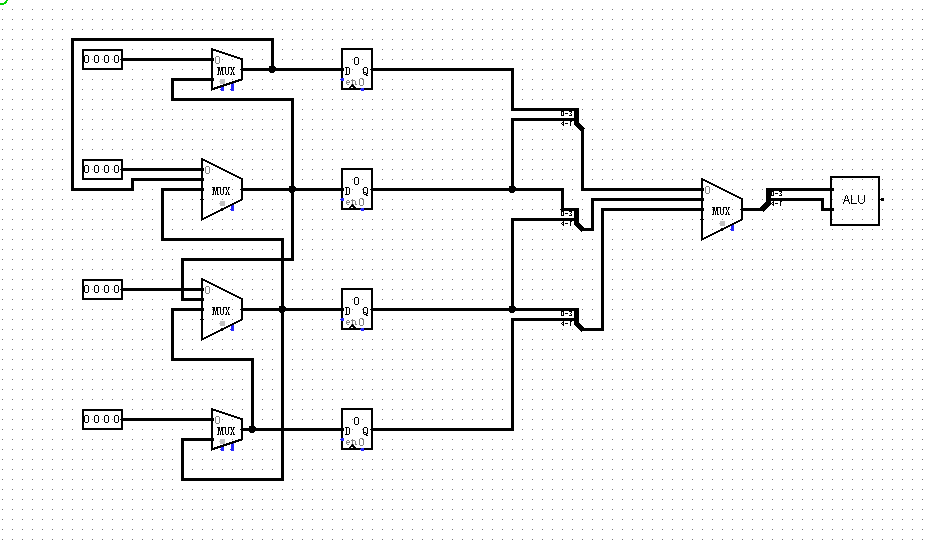
\includegraphics[scale=0.5]{circuit.png}
\end{figure}\par
\begin{lstlisting}[language=verilog]
// Data Path
//// mux
////// 用于交换的mux
mux2 mux2_0(.select(m0), .in0(x0), .in1(s1), .out(i0));
mux3 mux3_1(.select(m1), .in0(x1), .in1(s0), .in2(s2), .out(i1));
mux3 mux3_2(.select(m2), .in0(x2), .in1(s1), .in2(s3), .out(i2));
mux2 mux2_3(.select(m3), .in0(x3), .in1(s2), .out(i3));
////// 用于输入到ALU的mux
mux3 #(.WIDTH(2*N)) mux_ab(.select(mab), .in0({s0, s1}), .in1({s1, s2}), .in2({s2, s3}), .out({alu_a, alu_b}));
//// register
register register0(.data(i0), .en(en0), .rst(rst), .clk(clk), .r(s0));
register register1(.data(i1), .en(en1), .rst(rst), .clk(clk), .r(s1));
register register2(.data(i2), .en(en2), .rst(rst), .clk(clk), .r(s2));
register register3(.data(i3), .en(en3), .rst(rst), .clk(clk), .r(s3));
//// ALU
ALU ALU(.a(alu_a), .b(alu_b), .m(SUB), .cf(cf));
\end{lstlisting}

\subsubsection{状态机控制}
按照冒泡排序的过程, 有如下状态机控制.
\begin{lstlisting}[language=verilog]
// Control Unit
always @(posedge clk or posedge rst)
begin
    if(rst) cur_state <= LOAD;
    else cur_state <= next_state;
end

// States
always @(*)
begin
    case(cur_state)
        LOAD: next_state = CX01_3;
        CX01_3: next_state = CX12_3;
        CX12_3: next_state = CX23_3;
        CX23_3: next_state = CX01_2;
        CX01_2: next_state = CX12_2;
        CX12_2: next_state = CX01_1;
        CX01_1: next_state = HLT;
        HLT: next_state = HLT;
        default: next_state = HLT;
    endcase
end
\end{lstlisting}
其状态转移图大致如下:
\begin{figure}[H]
	\centering
	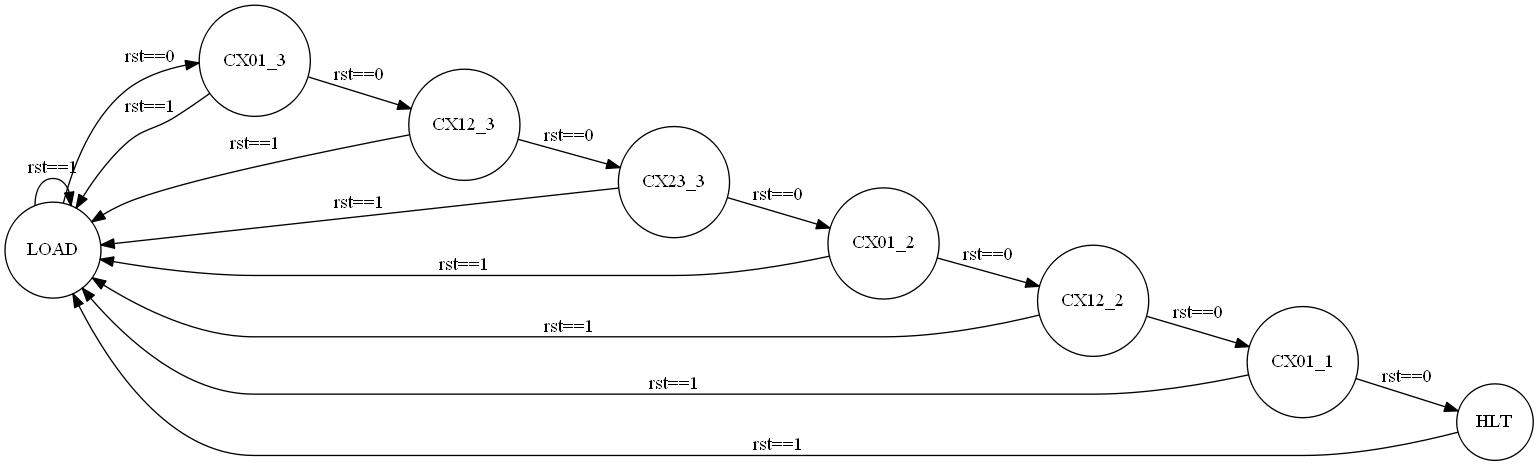
\includegraphics[scale=0.3]{graph.png}
\end{figure}\par
\subsubsection{控制单元}
这一部分是对数据交换的使能, 对ALU输入的选择等. 其中mx表示对x的选择; enx表示对x寄存器的使能; CXab\_i表示第i轮中对寄存器a和b的比较与交换.
\begin{lstlisting}[language=verilog]
always @(*)
begin
    // 初始化
    {mab, m0, m1, m2, m3, en0, en1, en2, en3, done} = 13'h00;
    case(cur_state)
        LOAD:
        begin
            {en0, en1, en2, en3} = 4'b1111;
        end
        CX01_3, CX01_2, CX01_1:
        begin
            mab = 2'b00;
            en0 = ~(y[N-1] ^ of); en1 = ~(y[N-1] ^ of);
            m0 = 1'b1; m1 = 2'b01;
        end
        CX12_3, CX12_2:
        begin
            mab = 2'b01;
            en1 = ~(y[N-1] ^ of); en2 = ~(y[N-1] ^ of);
            m1 = 2'b10; m2 = 2'b01;
        end
        CX23_3:
        begin
            mab = 2'b10;
            en2 = ~(y[N-1] ^ of); en3 = ~(y[N-1] ^ of);
            m2 = 2'b10; m3 = 1'b1;
        end
        HLT: done = 1'b1;
    endcase
end
\end{lstlisting}

\section{实验结果}
\subsection{ALU}
用老师给出的testbench可以得到如下波形图,
\begin{figure}[H]
	\centering
	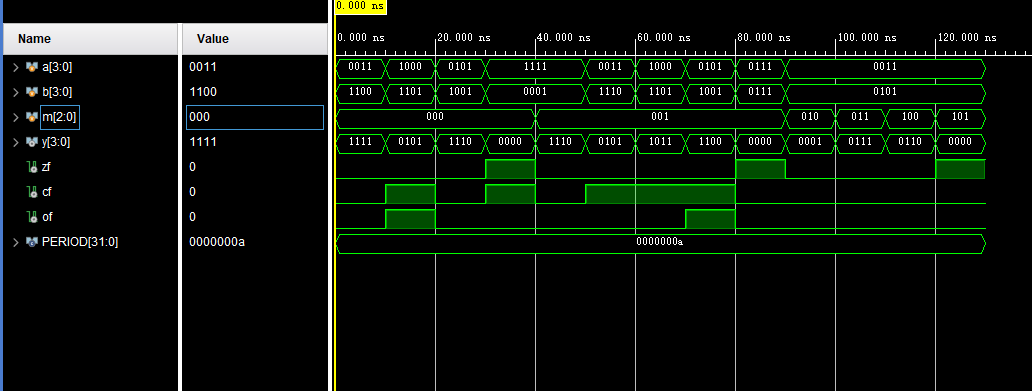
\includegraphics[scale=0.5]{alu_sim.png}
\end{figure}\par
可以看到当m为000时的加法, 为001时的减法等都得到了相应的正确结果.\par
而对于m=101的情况, 则默认对\{cf, y\}赋值为\{(WIDTH+1)\{1'b0\}\}, 其余的仍按原过程实现.

\subsection{sort}
由于老师给出的testbench只有3个数据, 于是自己编写了一个testbench, 随机生成4个数来排序. 仿真结果如下:
\begin{figure}[H]
	\centering
	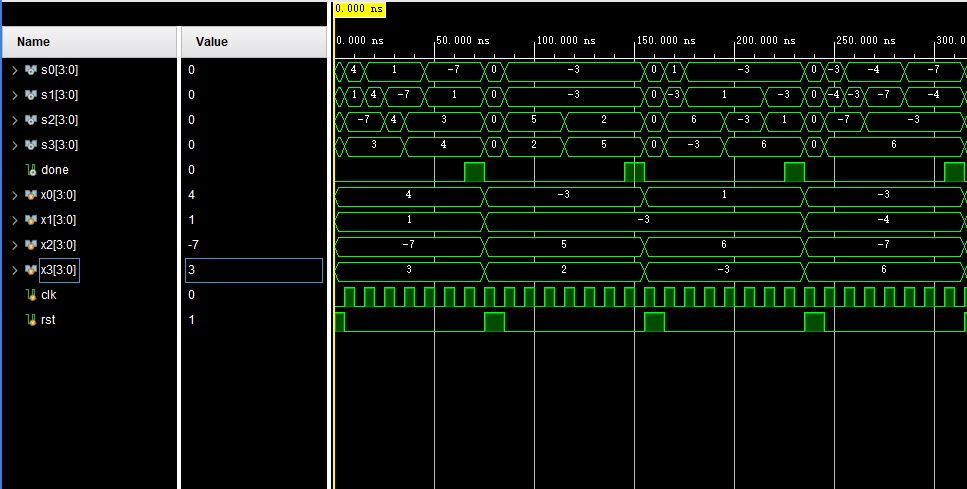
\includegraphics[scale=0.5]{sort_sim.png}
\end{figure}
其中sx显示为0的部分是rst的结果. 可以看到每组输入数据最终都完成了从小到大的有符号排序.

\section{思考题}
\subsection{如果要求排序后的数据是递减顺序,电路如何调整?}
递减顺序的话, 直接将输入ALU的两个操作数对调即可.
\subsection{如果为了提高性能,使用两个ALU,电路如何调整?}
可以使用奇偶并行排序算法. 先比较交换第1,2个和第3,4个; 再第2,3个; 再第1,2个和第3,4个.\par
这时s1,s2,s3,s4就变为有序的了.\par

\section{心得体会}
本次实验完成了ALU的设计, 这对后期设计CPU将有很大帮助. 此外这个排序器的实现方式, 让我回忆起了状态机的设计流程.

\section{意见建议}
本次实验相对简单,没有什么意见建议。\par
但希望老师讲课的网络环境可以得到改善,否则时不时就卡一下,很影响效率。

\end{document}






